\documentclass[10pt,twocolumn,letterpaper]{article}

\usepackage{cvpr}
\usepackage{times}
\usepackage{epsfig}
\usepackage{graphicx, color, xcolor}
\usepackage{amsmath}
\usepackage{amssymb}
\usepackage{bm}
\usepackage[utf8]{inputenc}
\usepackage{fancyhdr}
\usepackage{graphicx}
\usepackage[brazil]{babel}
\usepackage{lipsum}
\usepackage{float}
\setlength{\headheight}{1.5cm}

\fancypagestyle{plain}
\lhead{
\includegraphics[width=5cm,height=2cm]{logoFT.png}}
\rhead{
\includegraphics[width=5cm,height=2cm]{logoUnB.png}}

\renewcommand{\headrulewidth}{1pt}%
}

% Changing the caption and 'References' names to Portuguese.
\addto\captionsenglish{
  \renewcommand{\figurename}{Figura}
  \renewcommand{\tablename}{Tabela}
  \renewcommand{\refname}{Referências bibliográficas}
}

% to-do: Using fontenc with T1 font encoding allows \hyphenation to take words with accents
% as arguments. However, fontenc with T1 mess up with words containing 'ã' in all \subsection{}
% commands.
% If someone knows how to fix it, tell me!
%
%\usepackage[T1]{fontenc}

% Put the words not correctly hyphenated down here. Words with accents must
% be manually hyphenated in the text itself using the '\-' separator. See the examples
% throughout this template.
\hyphenation{co-e-ren-te u-sa-do de-li-mi-ta-do-res a-cer-ca va-lo-res cor-res-pon-den-te re-fe-ren-ci-a-das co-lu-na co-lu-nas em-bo-ra u-ti-li-da-de pro-ce-di-men-to ex-pe-ri-men-to fi-gu-ras}

% If you comment hyperref and then uncomment it, you should delete
% egpaper.aux before re-running latex.  (Or just hit 'q' on the first latex
% run, let it finish, and you should be clear).
\usepackage[breaklinks=true,bookmarks=true]{hyperref}

\cvprfinalcopy % *** Uncomment this line for the final submission

%\def\cvprPaperID{****} % *** Enter the CVPR Paper ID here
%\def\httilde{\mbox{\tt\raisebox{-.5ex}{\symbol{126}}}}

% Pages are numbered in submission mode, and unnumbered in camera-ready
% \ifcvprfinal\pagestyle{empty}\fi
%\setcounter{page}{1}


\begin{document}
%%%%%%%%% TITLE
\title{Experimento 2: Simulações com Amplificadores Operacionais}

\author{Yuri Shumyatsky\\
% To save space, use either the email address or home page, not both
{\tt\small 231012826@aluno.unb.br}\\
% Matrícula do primeiro autor
{\tt\small 231012826}\\
% Turma
{\tt\small Turma T02}
}

\maketitle
%\thispagestyle{empty}

%%%%%%%%% OBJETIVO

\begin{objetivo}
% Resumo com não mais de 250 palavras.
O experimento tem por objetivo difundir o entendimento sobre como funcionam os amplificadores operacionais e suas diversas configurações, como a não inversora, a inversora, buffer e diferencial. Além disso, os circuitos foram simulados no software LTspice de forma a demonstrar que todos os conceitos estudados (curto virtual, a necessidade de alimentação externa, entre outros) são válidos. 

\end{objetivo}

%%%%%%%%% BODY TEXT
\section{Introdução}

Os amplificadores operacionais (amps. ops.) são dispositivos eletrônicos fundamentais na área de eletrônica analógica, amplamente utilizados em diversas aplicações como amplificação de sinais, filtros ativos, circuitos matemáticos e instrumentação. Devido à sua alta versatilidade, permitem a implementação de uma grande variedade de configurações, cada uma com propriedades específicas de ganho, impedância e resposta em frequência.

Neste experimento, buscou-se explorar algumas das configurações mais comuns de amplificadores operacionais, a saber: inversora, não inversora, buffer (seguidor de tensão), integradora e amplificadora de diferença. Além de observar experimentalmente os efeitos de cada uma dessas configurações, também foi possível verificar fenômenos intrínsecos ao funcionamento dos amps. ops., como a existência do curto virtual, a saturação da saída quando a tensão excede os limites de alimentação e as propriedades de impedância de entrada e saída.

A simulação foi realizada no software LTspice, que possibilita analisar de forma prática e visual o comportamento dos circuitos, reforçando a teoria estudada em sala de aula. Os resultados obtidos permitem compreender não apenas o funcionamento ideal dos amps. ops., mas também os efeitos não ideais inerentes aos modelos reais utilizados.

\section{Fundamentação teórica}

O amplificador operacional ideal é um dispositivo de ganho infinito, com impedância de entrada infinita e impedância de saída nula. Na prática, esses valores são limitados, mas ainda suficientemente elevados para que os conceitos básicos de projeto se mantenham válidos.

A seguir, são apresentadas as configurações estudadas:

\begin{itemize}
    \item \textbf{Amplificador inversor}: Nesta configuração, a entrada é aplicada ao terminal inversor através de um resistor $R_1$, enquanto o resistor $R_2$ faz a realimentação negativa. O ganho é dado por:
    \[
    G = -\frac{R_2}{R_1}
    \]
    A saída é defasada de $180^\circ$ em relação à entrada.

    \item \textbf{Amplificador não inversor}: A entrada é aplicada ao terminal não inversor, enquanto o divisor resistivo ($R_1$ e $R_2$) faz a realimentação no terminal inversor. O ganho é:
    \[
    G = 1 + \frac{R_2}{R_1}
    \]
    A saída está em fase com a entrada e apresenta elevada impedância de entrada.

    \item \textbf{Buffer (seguidor de tensão)}: É o caso particular do amplificador não inversor com $R_1 \to \infty$ e $R_2 = 0$, resultando em ganho unitário ($G=1$). Sua principal utilidade é isolar estágios de circuito, devido à alta impedância de entrada e baixa impedância de saída.

    \item \textbf{Integrador}: Obtido substituindo $R_2$ por um capacitor $C$ no circuito inversor. A saída passa a ser proporcional à integral da entrada:
    \[
    V_{out}(t) = -\frac{1}{R_1 C} \int V_{in}(t) \, dt
    \]
    Por exemplo, para uma entrada quadrada, a saída será uma forma de onda triangular.

    \item \textbf{Amplificador de diferença}: Essa configuração amplifica a diferença entre dois sinais de entrada, sendo sua equação:
    \[
    V_{out} = \frac{R_2}{R_1}(V_2 - V_1)
    \]
    quando os resistores estão devidamente casados. Essa configuração é base para amplificadores de instrumentação e sistemas de rejeição de ruído em modo comum.
\end{itemize}

Além dessas configurações, o estudo também permite observar fenômenos importantes como a \textbf{saturação}, que ocorre quando $V_{out}$ tenta ultrapassar os limites impostos pelas tensões de alimentação do amp. op., e o \textbf{curto virtual}, conceito essencial em que os terminais de entrada (inversor e não inversor) apresentam praticamente o mesmo potencial em regime linear, devido ao ganho elevado do dispositivo.



%-------------------------------------------------------------------------


%-------------------------------------------------------------------------
\section{Simulações}

\subsection{Importação de Componentes}
Foi feita a importação do modelo SPICE do amp. op. \textbf{MC1458} e montado com ele um amplificador inversor, com $R_1 = 1k\Omega$ e $R_2 = 3k\Omega$, valores escolhidos para que o ganho seja $|G|=3$. Como sabemos, para essa configuração o ganho é de $G = -\frac{R_2}{R_1}$. 

\begin{figure}[h]
\caption{Circuito inversor com MC1458}
\begin{center}
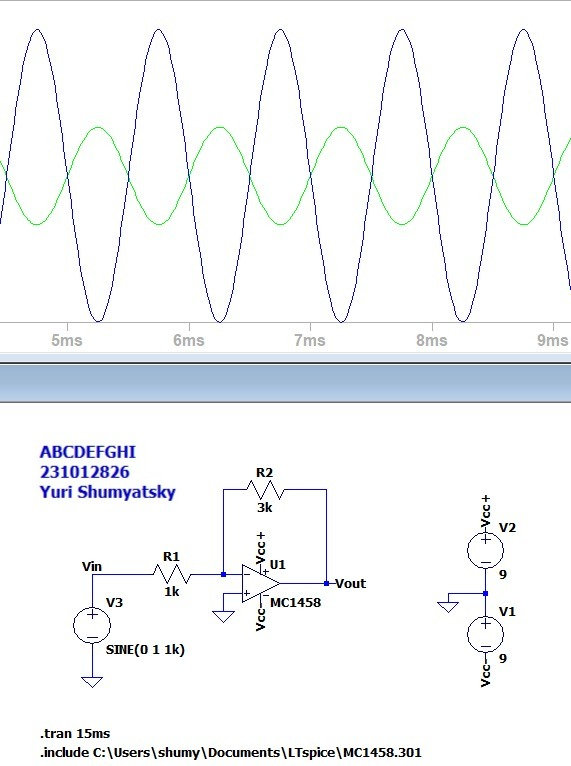
\includegraphics[scale=0.27]{figuras/fig1}
\end{center}
\end{figure}

\subsection{Circuito inversor}

Foi montado o circuito inversor com $R_1=31k\Omega$, $R_2=1k\Omega$ e alimentado por tensões de $\pm20V$. Primeiro, a entrada é dada como uma senoide de 28Hz e amplitude de 0.26V

\begin{figure}[h]
\caption{Circuito inversor com LM741}
\begin{center}
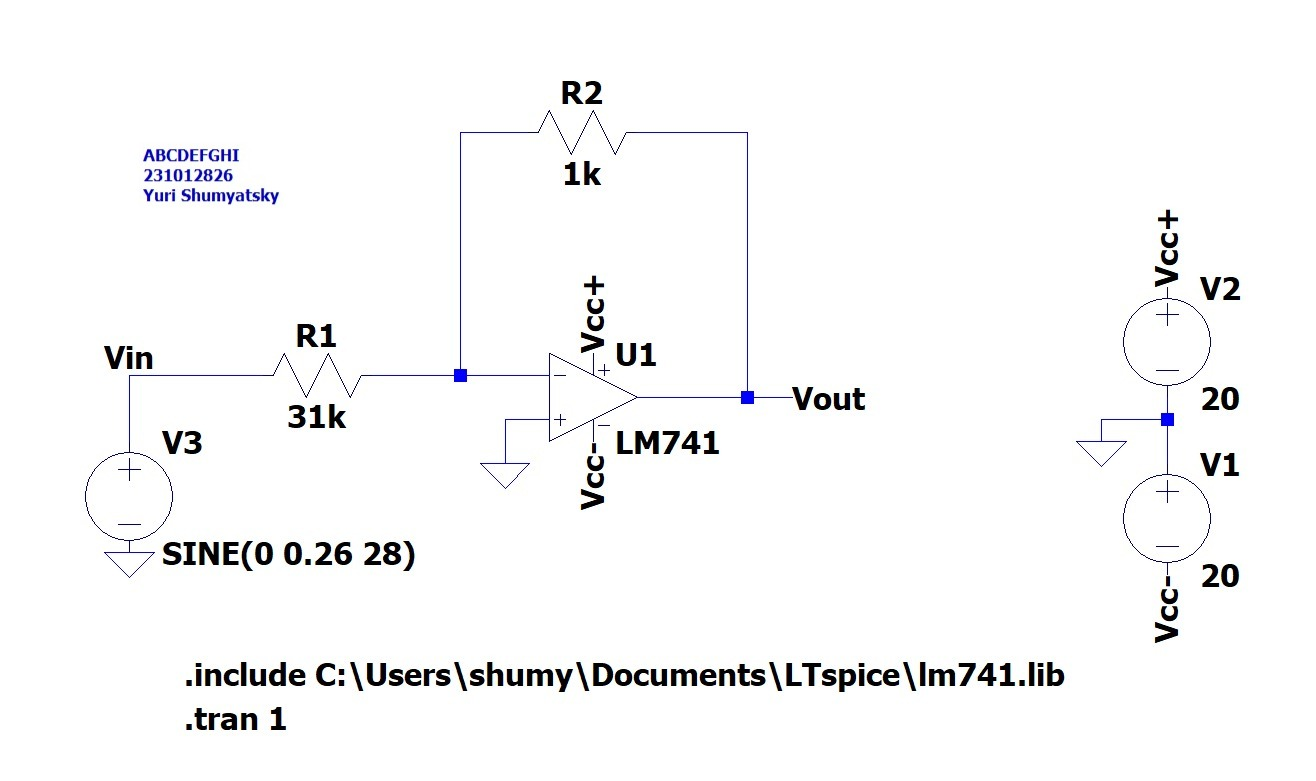
\includegraphics[scale=0.15]{figuras/fig2}
\end{center}
\end{figure}
\newpage

\begin{figure}[h]
\caption{Saída do circuito inversor}
\begin{center}
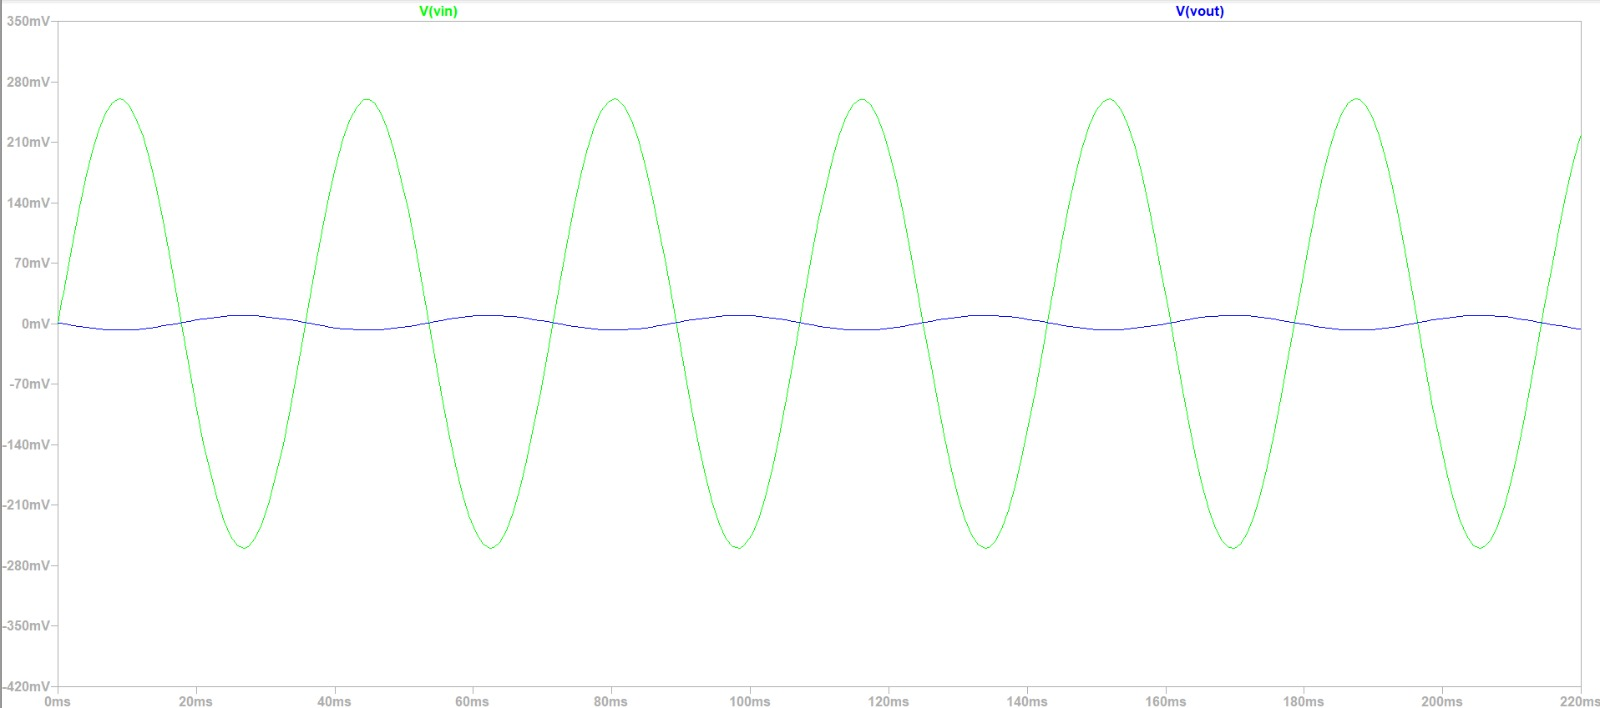
\includegraphics[scale=0.15]{figuras/fig3}
\end{center}
\end{figure}

Como esperado, de fato o ganho é baixo, de -0.0322.

Foram medidas as tensões nos pinos 2 e 3, no entanto o pino 3 está conectado diretamente ao GND e portanto não sua tensão não pôde ser plotada. 

\begin{figure}[h]
\caption{Tensão pino 2}
\begin{center}
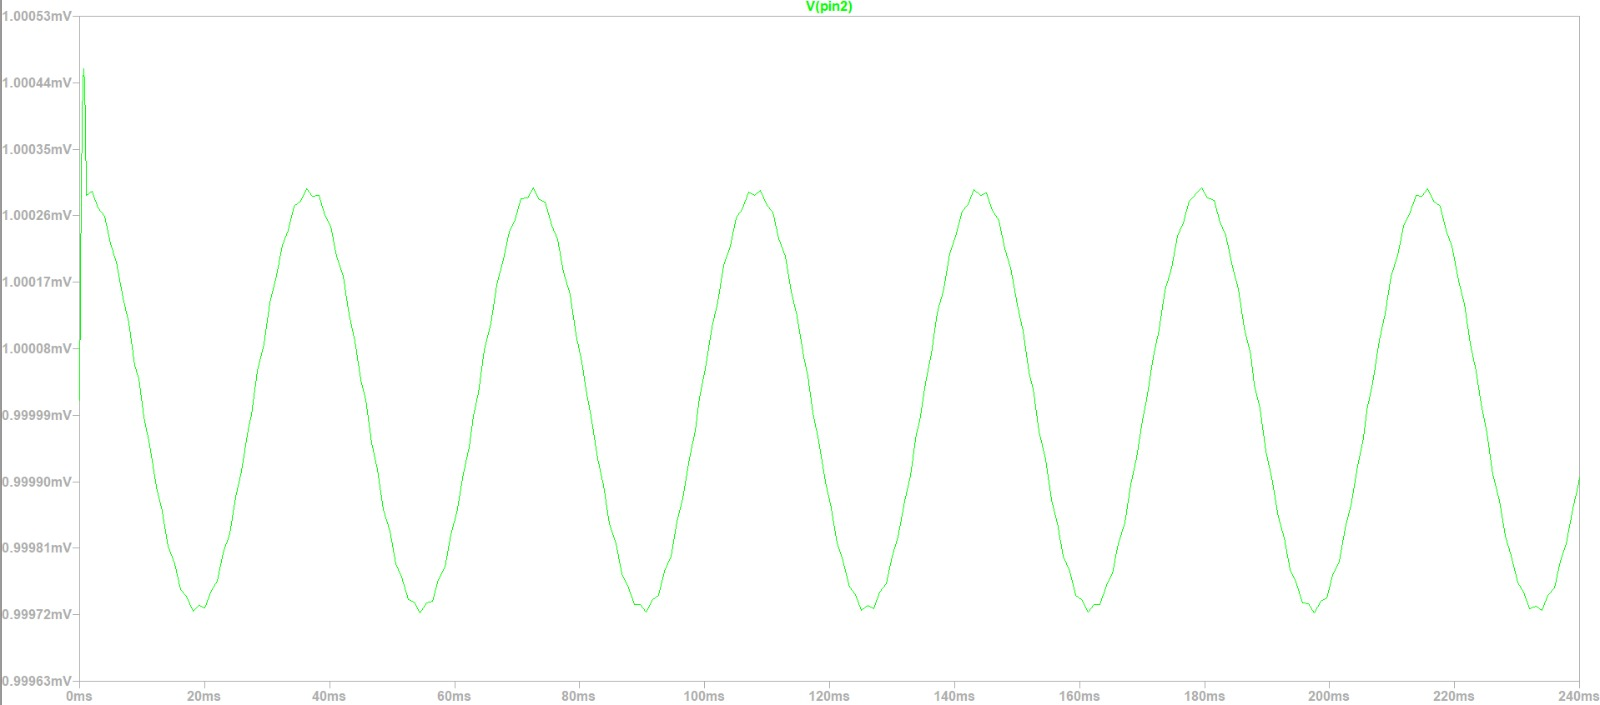
\includegraphics[scale=0.15]{figuras/fig4}
\end{center}
\end{figure}

A tensão é baixa, tendo amplitude máxima de aproximadamente 1mV. De fato, o esperado é que V+ e V- sejam iguais para que haja o curto virtual, mas como o componente não é ideal, esse é o resultado.

Aumentando a tensão gradualmente, nada acontece até $V_{out}$ chegar em 20V de amplitude (a tensão de $V_{cc}$), em que a saturação começa a fazer efeito. Isso acontece com $V_{in}$ tendo amplitude de 620V.
\newpage

\begin{figure}[h]
\caption{Saturação}
\begin{center}
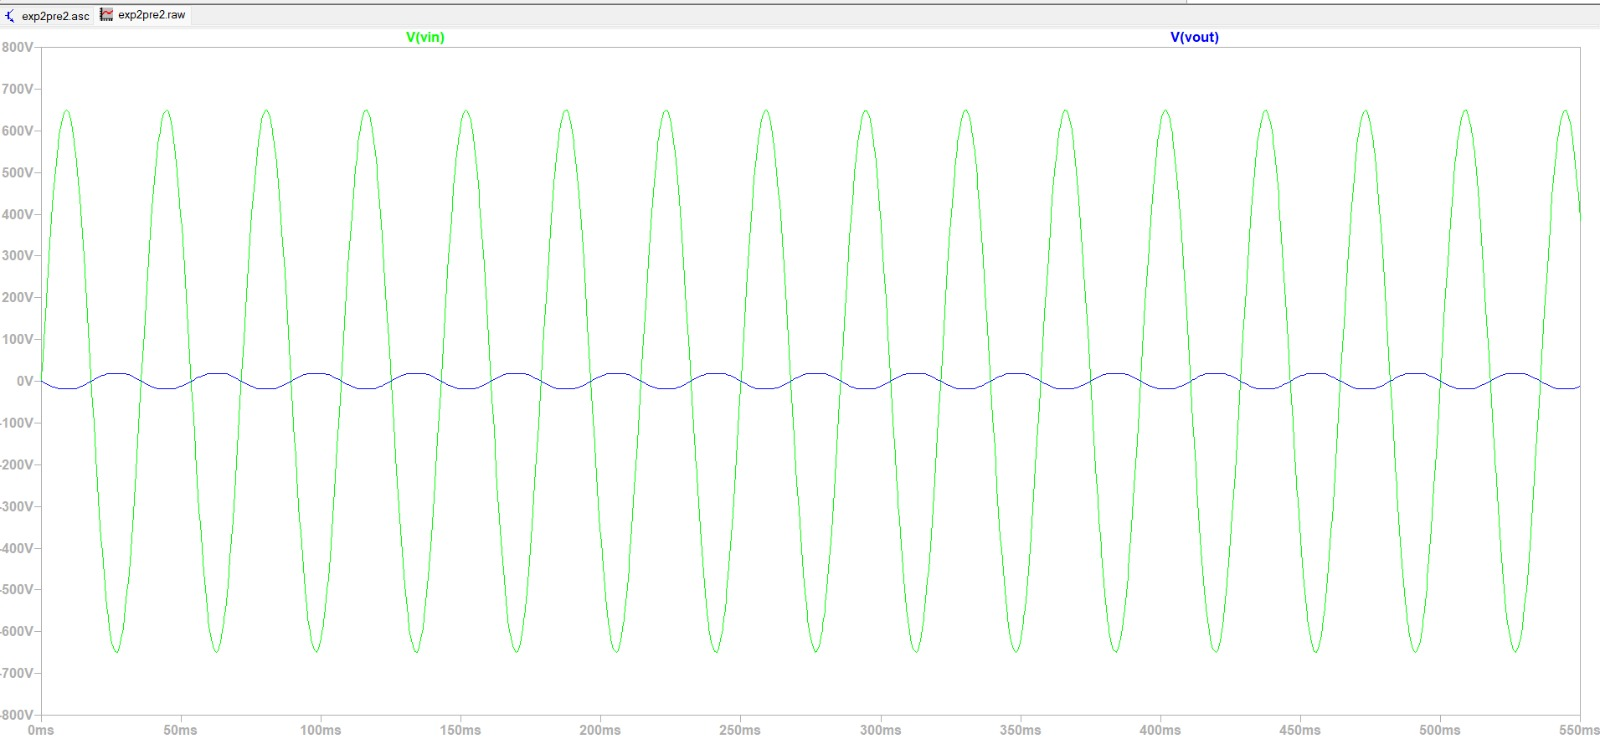
\includegraphics[scale=0.15]{figuras/fig5}
\end{center}
\end{figure}

Substituindo $R_2$ por um capacitor e a entrada por uma onda quadrada de amplitude 10V e período de 20ms, obtemos a seguinte curva: 

\begin{figure}[h]
\caption{Substituição para onda quadrada e capacitor}
\begin{center}
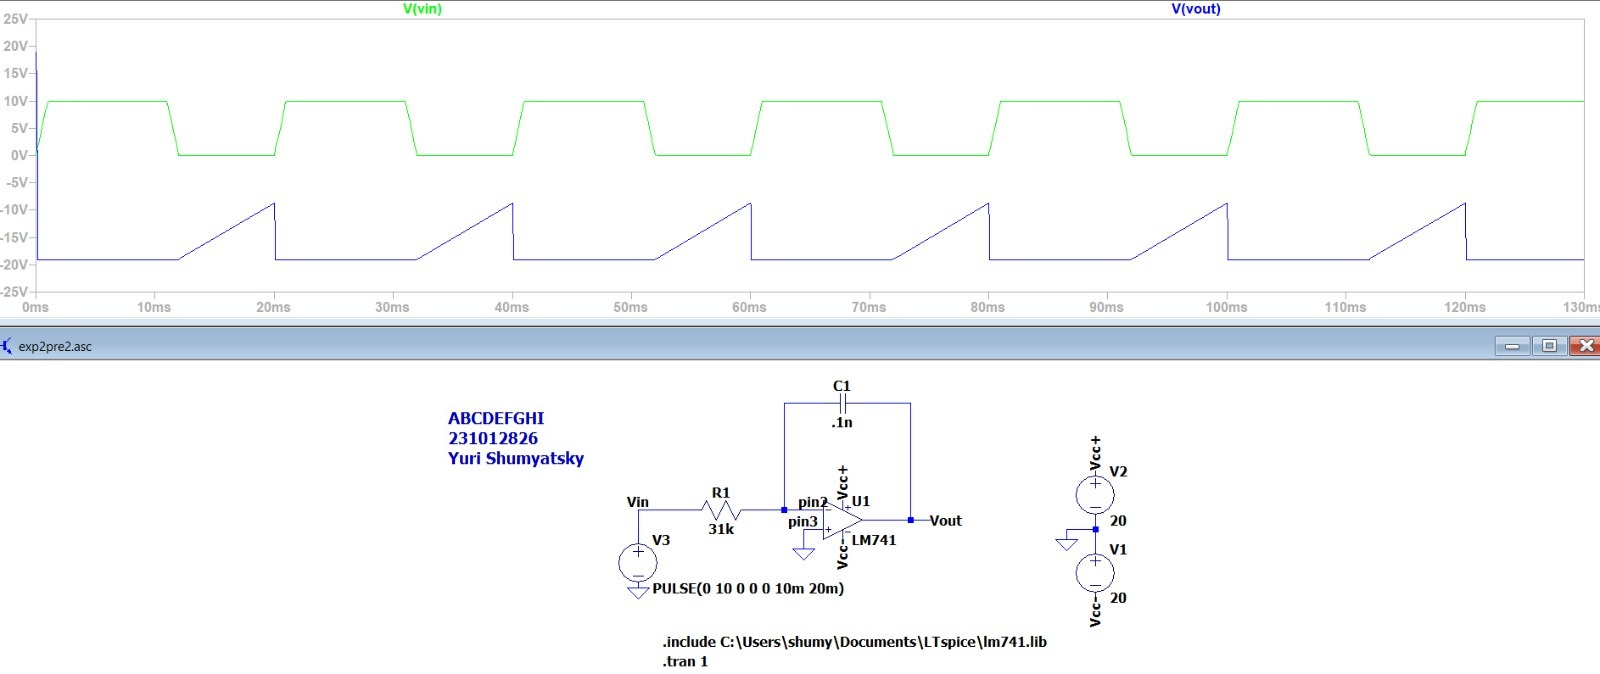
\includegraphics[scale=0.15]{figuras/fig6}
\end{center}
\end{figure}

Essa configuração é conhecida como integrador, e de fato a integral deve ser uma onda triangular. Essa simulação foi realizada com 0.1nF. Diminuindo a capacitância para 0.005nF, obtemos a seguinte curva saturada:

\begin{figure}[h]
\caption{Diminuição da capacitância}
\begin{center}
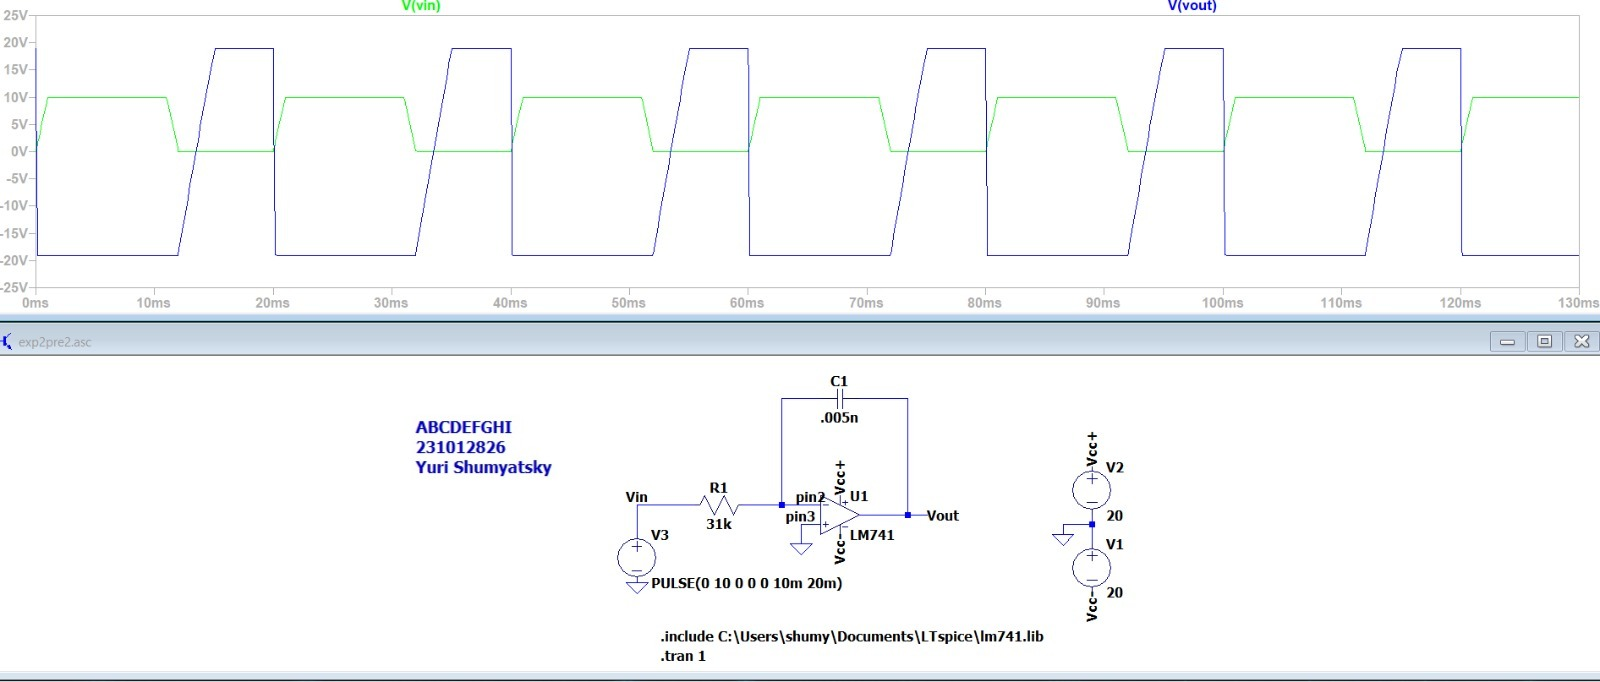
\includegraphics[scale=0.15]{figuras/fig7}
\end{center}
\end{figure}

\newpage
\subsection{Amplificador Não-Inversor}

A configuração do circuito agora muda:

\begin{figure}[h]
\caption{Circuito Não-Inversor}
\begin{center}
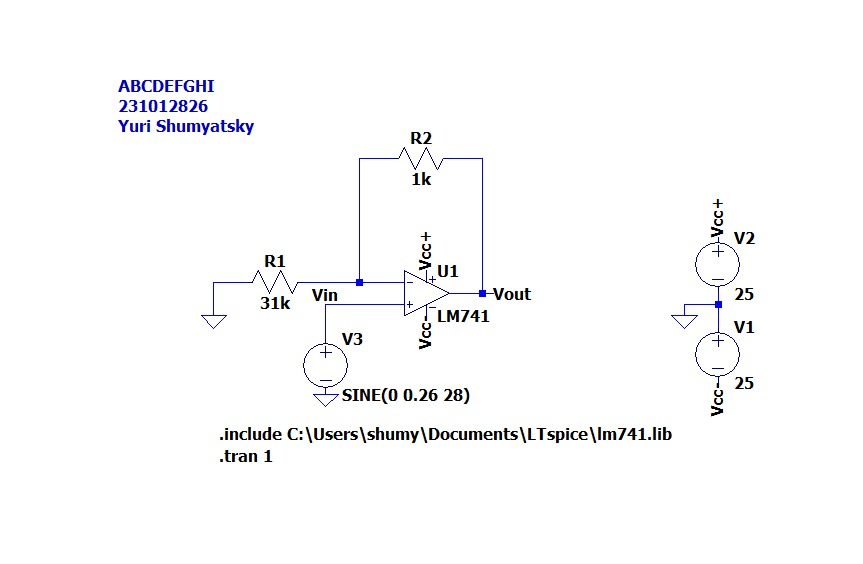
\includegraphics[scale=0.2]{figuras/fig8}
\end{center}
\end{figure}

Usamos $R_1 =  31k\Omega$, $R_2=1k\Omega$, o amplificador operacional é alimentado por fontes de $\pm25V$. Com uma entrada senoidal de 28Hz e amplitude de 0.26V, obtemos as seguintes plotagens para a entrada e saída:

\begin{figure}[h]
\caption{Tensões Não-Inversor}
\begin{center}
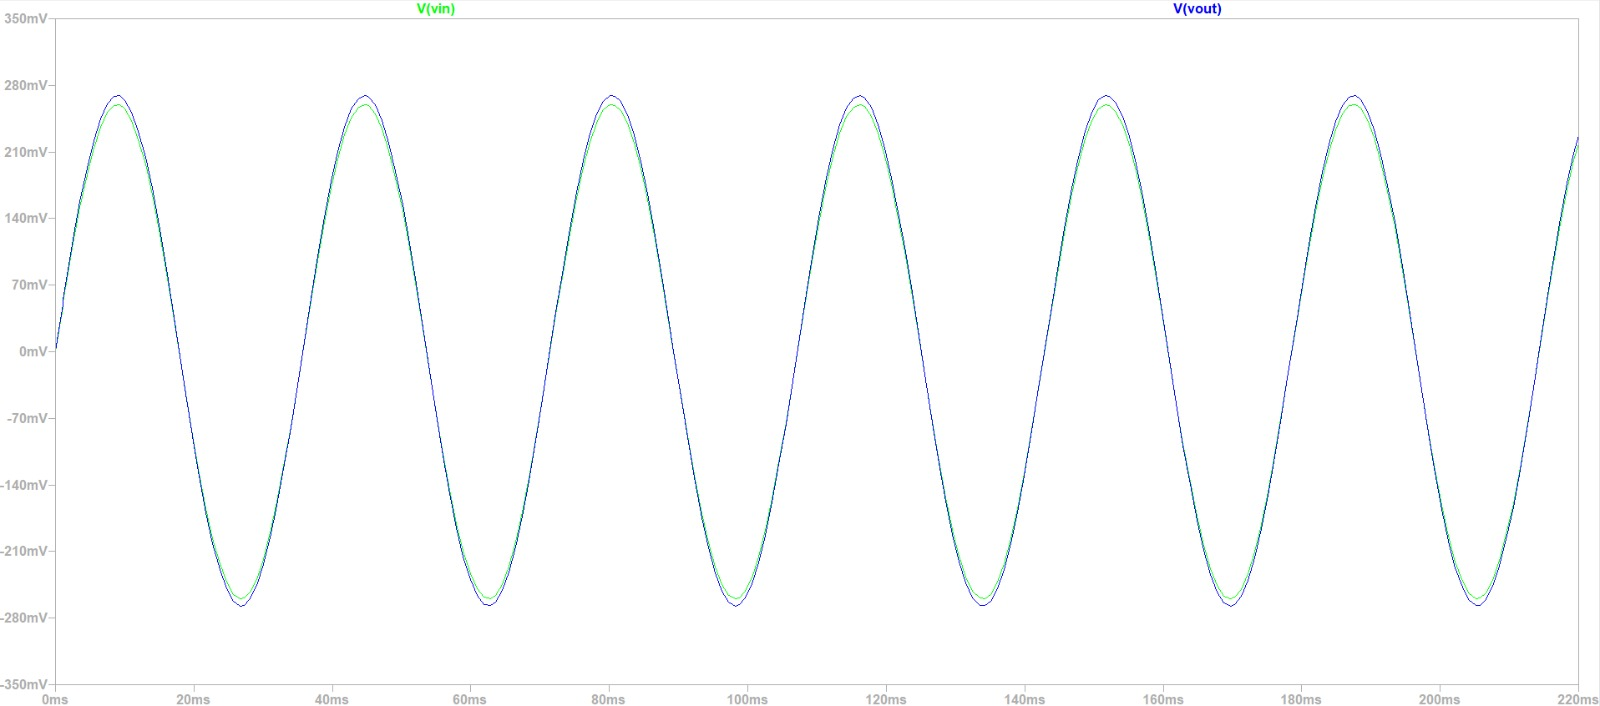
\includegraphics[scale=0.15]{figuras/fig9}
\end{center}
\end{figure}

Como esperado, o ganho é de 1.0322, e portanto as tensões são muito próximas.

Para verificar que a impedância de entrada é alta, foi adicionado uma resistência de $1k\Omega$ entre a $V_in$ e a entrada não inversora do amp. op., e a corrente nessa resistência é medida, tendo um valor extremamente baixo, comprovando assim a hipótese.

Medindo as tensões dos pinos 2 e 3 para comprovar o curto virtual, obtemos novamente que um dos pinos está conectado no GND e por isso não é possível plotar a sua tensão, enquanto a outra tensão apresenta amplitude baixa. 

\newpage
\begin{figure}[h]
\caption{Tensões Pinos amp. op.}
\begin{center}
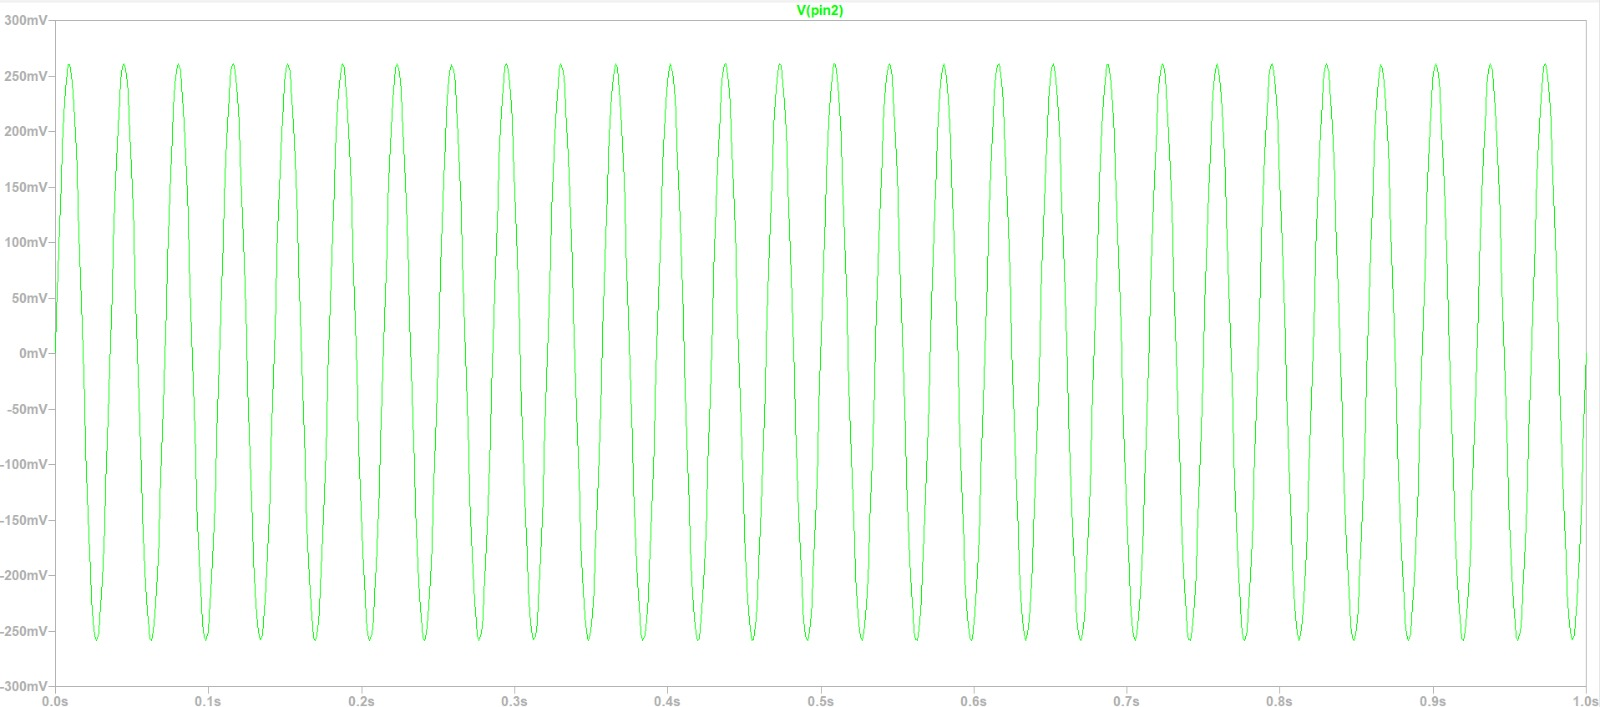
\includegraphics[scale=0.15]{figuras/fig10}
\end{center}
\end{figure}


\subsection{Buffer}

Novamente a configuração é alterada, dessa vez sem resistências mas com entrada senoidal de frequência 28Hz e amplitude 0.26V. 

\begin{figure}[h]
\caption{Circuito Buffer}
\begin{center}
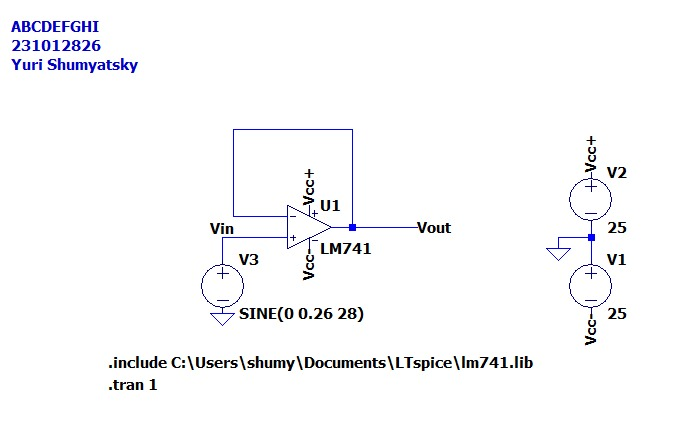
\includegraphics[scale=0.2]{figuras/fig11}
\end{center}
\end{figure}

Como o ganho é unitário, espera-se que a saída seja igual à entrada, o que de fato ocorre na simulação:

\begin{figure}[h]
\caption{Entrada e Saída Buffer}
\begin{center}
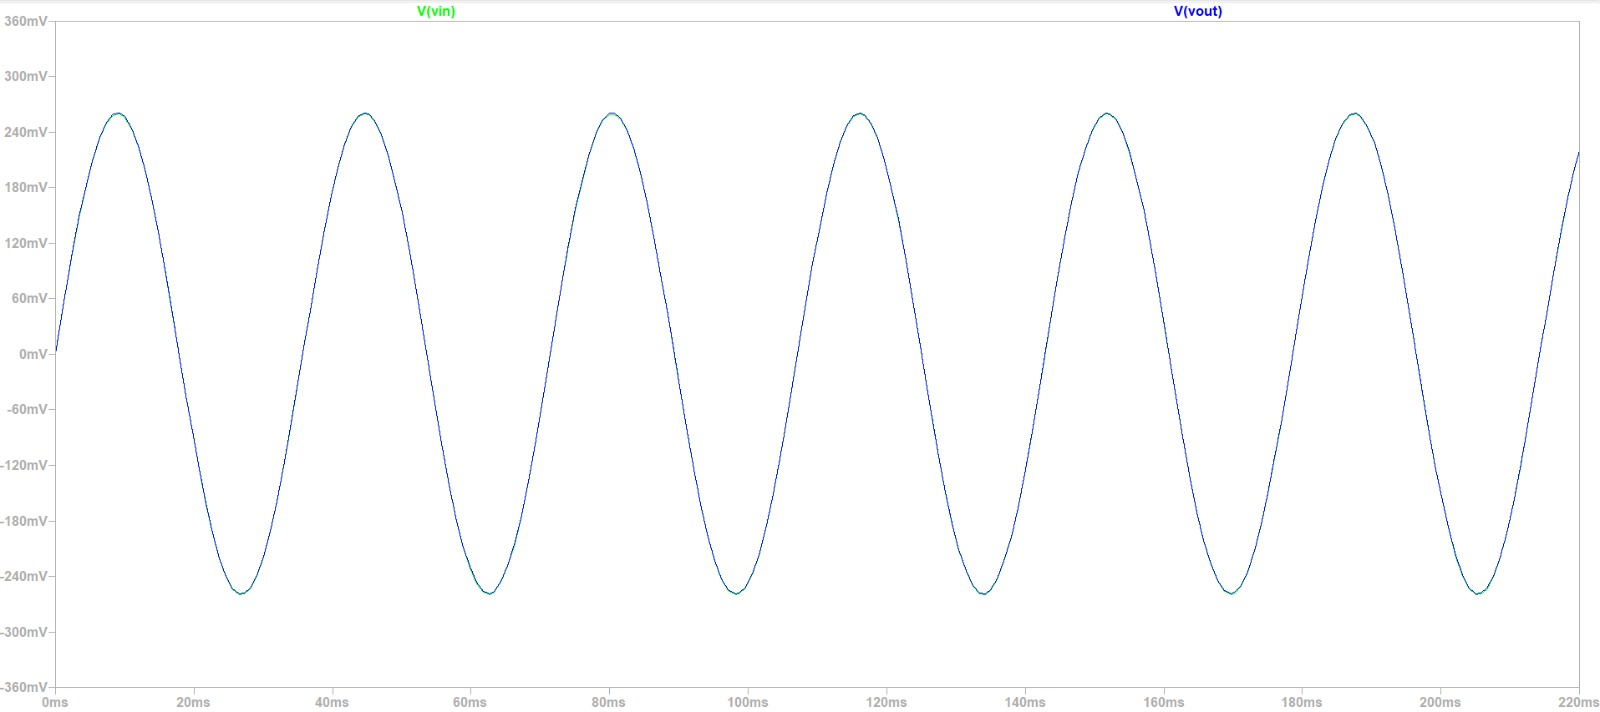
\includegraphics[scale=0.14]{figuras/fig12}
\end{center}
\end{figure}

Adicionando resistências de $31k\Omega$ e $1k\Omega$, 

\begin{figure}[h]
\caption{Buffer com resistências}
\begin{center}
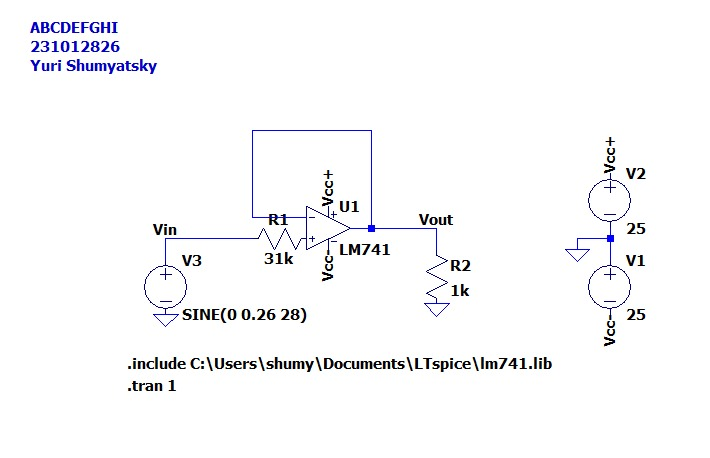
\includegraphics[scale=0.2]{figuras/fig13}
\end{center}
\end{figure}

Espera-se que a dissipação de tensão de $R_2$ seja a mesma de caso $R_1$ fosse igual a 0, na situação em que $R_1$ e $R_2$ estivessem em série. Isso é comprovado pela simulação, que mostra a amplitude de 260mV esperada. 

\begin{figure}[h]
\caption{Saída Buffer}
\begin{center}
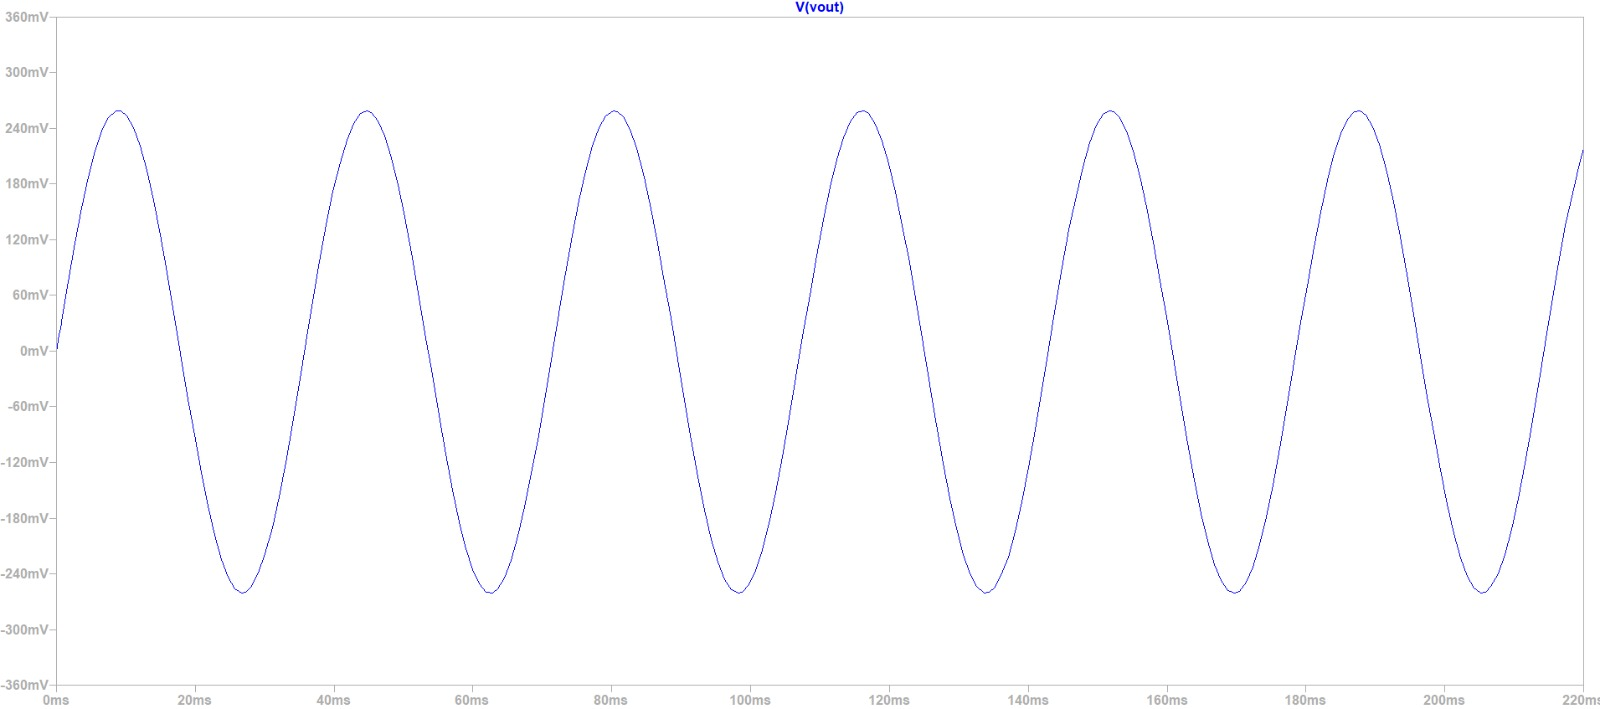
\includegraphics[scale=0.15]{figuras/fig14}
\end{center}
\end{figure}

\subsection{Amplificador de Diferença}

O circuito é montado com $R_1=31k\Omega$, $R_2=1k\Omega$, $V_1=1$ e $V_2=sin(40\pi t)$, i.e. frequência de 20 Hz.

\begin{figure}[h]
\caption{Amplificador de Diferença}
\begin{center}
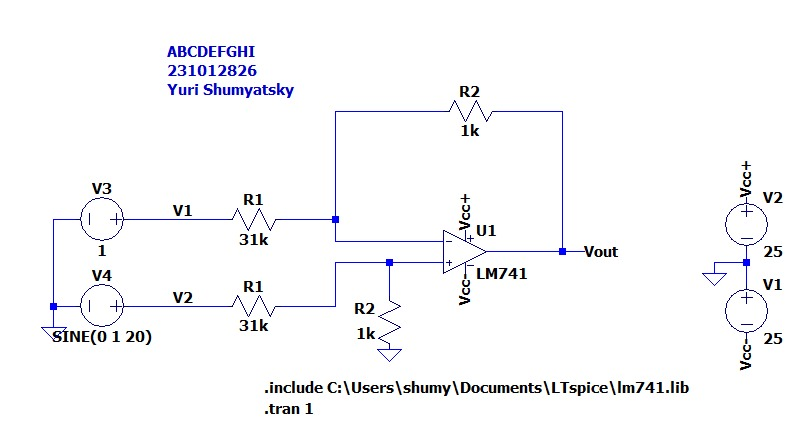
\includegraphics[scale=0.2]{figuras/fig15}
\end{center}
\end{figure}

Como esperado, a saída é proporcional a $V_1-V_2$.

\begin{figure}[h]
\caption{Saída Amplificador de Diferença}
\begin{center}
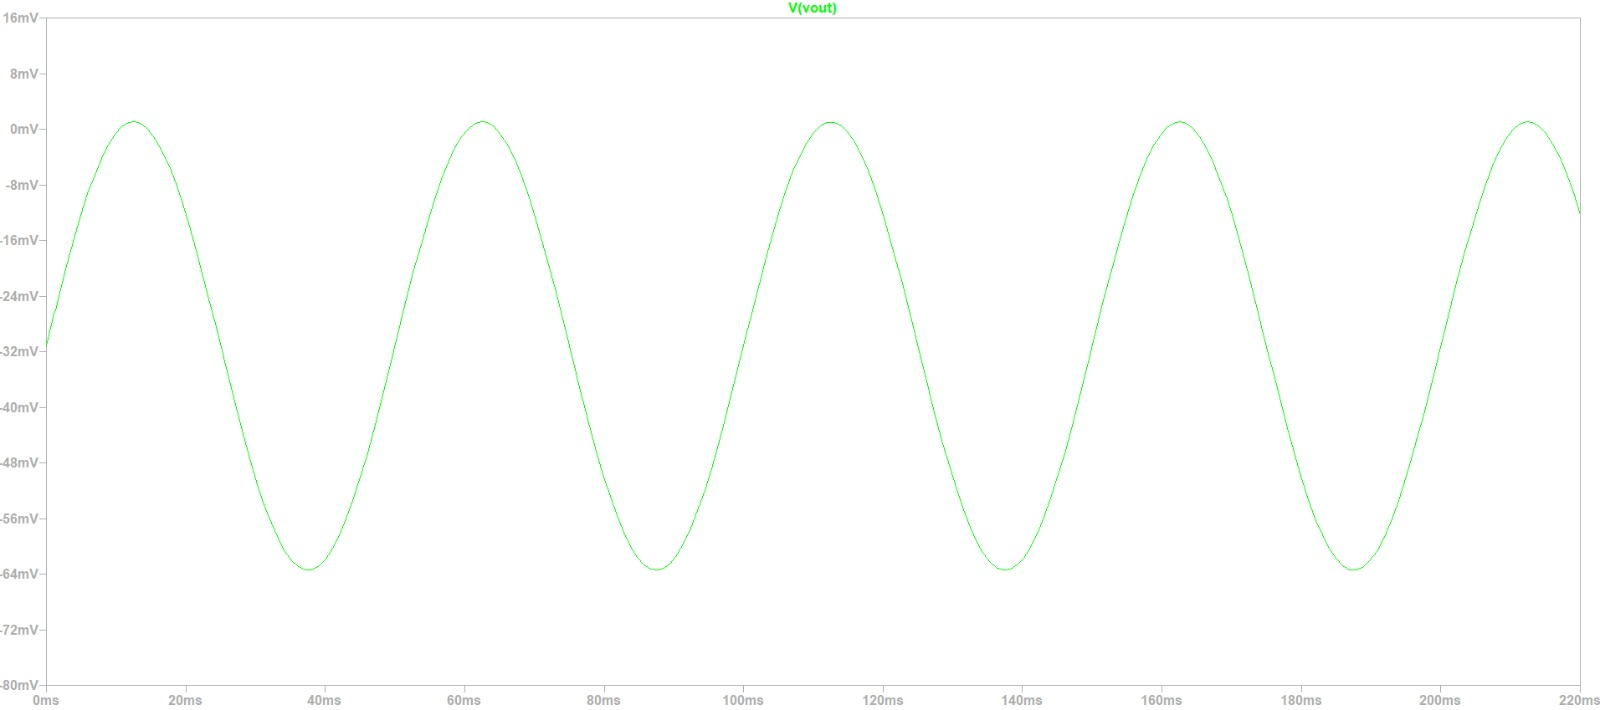
\includegraphics[scale=0.15]{figuras/fig16}
\end{center}
\end{figure}

%-------------------------------------------------------------------------


{\small
\bibliography{egbib}
\bibliographystyle{ieee_fullname}
}
\begin{itemize}
\item Razavi, B. Fundamentos de Microeletrônica, 2\textordfeminine Edição, LTC, 2014.
\end{itemize}

\end{document}
